\documentclass[11pt]{article}
\usepackage[a4paper,margin=25mm]{geometry}
\usepackage[T1]{fontenc}
\usepackage{lmodern,microtype}
\usepackage{amsmath,amssymb,amsthm,booktabs,graphicx,array}
\usepackage{xcolor,enumitem}
\usepackage[colorlinks=true,linkcolor=blue!45!black,citecolor=blue!45!black,urlcolor=blue!45!black]{hyperref}
\usepackage[font=small,labelfont=bf]{caption}
\setlength{\parskip}{3pt}
\setlength{\parindent}{1.2em}
\setlist{itemsep=2pt,topsep=4pt}
\newtheorem{proposition}{Proposition}
\newtheorem{theorem}{Theorem}
\newtheorem{corollary}{Corollary}
\newcommand{\A}{\mathcal A}
\newcommand{\E}{\mathcal E}
\newcommand{\infv}{+\infty}
\title{\textbf{When Does a Slower Escape Route Buy Useful Time?}\\[5pt]
\large Departure-Delay Guarantees and Small Route Menus\\in Flooding Networks}
\author{}
\date{Working preprint --- October 25, 2026}
\begin{document}
\maketitle
\begin{abstract}
An escape route optimized for immediate departure need not remain usable after a delayed notification. We study the cost of choosing a fixed route that remains feasible over a specified departure-time interval, and the related problem of preparing a small menu of routes for different flood locations. For prescribed FIFO tunnel-arrival functions with permanent closures, interval feasibility reduces to one endpoint condition. A two-departure label algorithm minimizes nominal arrival time subject to that condition; a backward calculation supplies infeasibility certificates and bounds for a travel-budget search. Small route menus are selected by exact maximum coverage within a training-derived candidate set and evaluated at withheld flood locations. Experiments use a competition network and a CAD-derived network, with a volume-accounting flood surrogate. Allowing 5\% extra nominal travel improves unrestricted departure tolerance at 63 of 80 sampled origins, but improves tolerance within a 60-minute horizon at none of them. Three-route menus increase held-out timely coverage from 94.77\% to 96.56\% on the competition network and from 97.26\% to 97.89\% on the CAD network, relative to a single nominal route. These modest gains, together with bottleneck certificates and sensitivity tests, show why a large mathematical delay margin need not be operationally useful. All numerical findings are conditional on the surrogate hazard schedules; they are not calibrated mine-safety predictions.
\end{abstract}

\section{Introduction}
Suppose an evacuation plan tells a miner to take the currently fastest route. The notification may arrive late, preparation may take longer than expected, or the assumed location of a water inrush may be wrong. Recomputing a shortest path after every change is one response. A different question arises when routes must be communicated or prepared in advance: how much immediate travel efficiency should be sacrificed to keep a fixed plan usable?

This study starts from the mine-inrush problem in the 2025 Contemporary Undergraduate Mathematical Contest in Modeling (CUMCM), Problem D \cite{cumcm}. The competition specifies tunnel networks, water-inrush scenarios, and notification times, and asks for flood propagation and escape plans. Its fastest-route formulation motivates the follow-up question studied here:
\begin{quote}
\emph{Given a bound on extra nominal travel time, how much additional departure delay can a fixed route tolerate, and how much of that tolerance falls within a relevant planning horizon?}
\end{quote}
We also ask whether two or three precomputed routes can cover several flood locations. These questions concern fixed routes and small route sets, rather than a new shortest-path calculation for each realized situation.

Three distinctions are essential. First, the latest feasible departure along a route is a model-relative \emph{availability deadline}, not a recommendation to wait underground. Second, a route that is fastest at a delayed departure need not minimize travel at the nominal departure while remaining feasible later. Third, the existence of a usable route in a menu does not imply that a miner can identify it from locally available information.

Our contribution is a precise formulation and reproducible investigation of these distinctions. We give an exact constrained-routing method, a certificate for when rerouting cannot increase delay tolerance, and a finite-scenario route-menu construction. The experiments reveal a limitation of the initial motivation: unrestricted delay gains can be dominated by very late modelled closures. We therefore report both unrestricted and horizon-capped improvements, including null results.

\paragraph{Relation to existing work.}
FIFO time-dependent shortest paths and the role of waiting have a substantial literature \cite{dean,orda}. Integrating time-dependent speeds, rather than freezing a travel time at entry, is an established way to preserve FIFO behavior \cite{ichoua}. Our label dominance argument specializes the multi-label principle used in multicriteria shortest paths \cite{martins}; it is not a claim to have invented a new general label-setting paradigm. Bounding deterioration of nominal quality while improving robustness is closely related to light robustness \cite{fischetti}. Recoverable robust routing instead permits a route to be updated after disruption \cite{goerigk}; the main optimization here keeps the route fixed. Route-menu selection is finite maximum coverage, whose submodular structure is classical \cite{nemhauser}. The contribution lies in the problem specification, the exact two-departure implementation, and the empirical separation of mathematical margin, relevant margin, and menu availability.

\section{A route has an arrival time and a departure deadline}
\label{sec:model}
Let $G=(V,\A)$ be a finite directed graph with origin $s$ and exit set $\E$. Each physical tunnel contributes two directed arcs. A prescribed hazard schedule assigns arc $e$ a length $L_e>0$, wetting time $w_e$, permanent closure time $b_e\ge w_e$, dry speed $v_0=4$ m/s, and wet speed $u_e\in\{1,2\}$ m/s. Wet speeds encode a fixed reference direction of water movement. The schedule is an input to routing, not a result of the routing algorithm.

For entry time $t$, define the exit time $A_e(t)$ by
\begin{equation}
 \int_t^{A_e(t)}v_e(\tau)\,d\tau=L_e,\qquad
 v_e(\tau)=
 \begin{cases}v_0,&\tau<w_e,\\u_e,&w_e\le\tau\le b_e.\end{cases}
 \label{eq:integral}
\end{equation}
If traversal cannot finish by $b_e$, set $A_e(t)=\infv$, and extend $A_e(\infv)=\infv$. Arrival exactly at closure is allowed; this is a mathematical convention, not a physical safety margin. The piecewise-constant speed makes the integral explicit. With $r=v_0\max(w_e-t,0)$,
\begin{equation}
 A_e(t)=
 \begin{cases}
 t+L_e/v_0,& L_e\le r,\\
 \max(t,w_e)+(L_e-r)/u_e,&L_e>r,
 \end{cases}
 \label{eq:forward}
\end{equation}
provided $t\le b_e$ and the displayed value does not exceed $b_e$.
For example, $L=20$ m, $w=4.1$ s, and $u=2$ m/s give $A_e(0)=5.9$ s. A 20-segment rule using speed at each segment's start gives 5.75 s. A closure at 5.77 s therefore reverses its feasibility verdict. Exact event integration avoids this discretization error.

For path $P=(e_1,\ldots,e_m)$, let $A_P=A_{e_m}\circ\cdots\circ A_{e_1}$. We stop a path when it first reaches an exit. A feasible path has finite $A_P(t)$. Define
\begin{equation}
 D(P)=\sup\{t:A_P(t)<\infv\},\qquad
 D^*(s)=\max_{P:s\to\E}D(P).
 \label{eq:deadline}
\end{equation}
These are absolute times measured from the start of the inrush. At nominal departure $t_0$, the available delay is $D(P)-t_0$. No congestion, fatigue, interaction between miners, or survival during pre-departure waiting is modelled.

\begin{proposition}[Endpoint reduction]
\label{prop:endpoint}
Each $A_e$ and $A_P$ is nondecreasing on extended real time. For $d\ge t_0$, a fixed path is feasible at every departure in $[t_0,d]$ if and only if it is feasible at $d$.
\end{proposition}
\begin{proof}
Two travelers using the same arc and direction have the same instantaneous speed whenever both are on that arc. The earlier entrant cannot be overtaken. If a later entrant completes before permanent closure, the earlier entrant also completes. Thus $A_e$ is nondecreasing, including the infeasible value $\infv$. Compositions preserve monotonicity, proving the path statement and the endpoint condition.
\end{proof}
For this model there is no benefit to waiting en route: leaving an arc earlier cannot worsen arrival downstream. Removing a cycle likewise cannot worsen either arrival time or feasibility. Hence a simple path suffices.

Let $P_0$ be a nominal earliest-arrival route and $T^*=A_{P_0}(t_0)-t_0$. We study
\begin{align}
 C(d)&=\min\{A_P(t_0):P:s\to\E,\ A_P(d)<\infv\}, \label{eq:C}\\
 D_\epsilon&=\max\{D(P):A_P(t_0)-t_0\le(1+\epsilon)T^*\}.
 \label{eq:budget}
\end{align}
An empty feasible set gives $C(d)=\infv$. Equal nominally optimal routes may have different deadlines, so $D_0$ is not necessarily the deadline of an arbitrary shortest-path tie-break. In the reported base experiments, no improvement above one second occurred at zero budget.

\section{Exact optimization at two departure times}
\subsection{Backward deadlines and an impossibility certificate}
For an arc whose downstream arrival must be at most $q$, define
$B_e(q)=\sup\{t:A_e(t)<\infv,\ A_e(t)\le q\}$.
Set $z=\min(q,b_e)$. In the present model,
\begin{equation}
 B_e(q)=
 \begin{cases}
 z-L_e/u_e,&z>w_e,\quad L_e\le u_e(z-w_e),\\
 \min(z,w_e)-[L_e-u_e\max(z-w_e,0)]/v_0,&\text{otherwise}.
 \end{cases}
 \label{eq:inverse}
\end{equation}
If $q=b_e=\infv$, define $B_e(q)=\infv$.
Applying these inverse maps backward along a fixed path computes $D(P)$ exactly.

For the whole graph, initialize exit labels to $\infv$ and all others to $-\infty$. Repeatedly settle the largest unsettled label and relax each incoming arc $(u,v)$ by
\[
 D(u)\leftarrow\max\{D(u),B_{uv}(D(v))\}.
\]
To see correctness, induct on settled nodes. If the next node had a later feasible departure, follow that route until it first enters the settled set. Its arrival there is bounded by the settled deadline, so the incoming edge would already have produced a candidate at least as large as the departure along the route. Since forward times never decrease, that candidate would exceed the label being settled, contradicting the maximum-label choice. The resulting label is $D^*(u)$. A heap implementation takes $O((|V|+|\A|)\log|V|)$ time.

\begin{corollary}[No-improvement certificate]
\label{cor:certificate}
If $D(P_0)=D^*(s)$, no fixed route, regardless of its nominal travel cost, tolerates a later departure than $P_0$.
\end{corollary}
This is a certificate within the prescribed schedule. It does not by itself identify a physical bridge or cut in the real mine.

\subsection{Why one clock is not enough}
Solving an ordinary earliest-arrival problem at $d$ minimizes $A_P(d)$, whereas \eqref{eq:C} minimizes $A_P(t_0)$ subject to feasibility at $d$. The objectives differ.

Consider two $s$--$v$ prefixes. The first is a 30 m arc, wet from 5 s, with wet speed 1 m/s. The second consists of two 36 m arcs that stay dry until 100 s. Their arrivals at $v$, for departures at 0 and 10 s, are respectively $(15,40)$ and $(18,28)$. Append a dry 20 m arc to the exit. If it closes at 100 s, both routes are feasible at the delayed departure: the first is nominally faster (20 versus 23 s), while the second is faster after delay (33 versus 45 s). If that last arc instead closes at 36 s, only the second prefix can be extended feasibly. Neither prefix can therefore be discarded on the basis of its nominal arrival alone.

\subsection{The two-departure label algorithm}
A label at node $v$ stores $(x,y)$, the arrival times of the \emph{same prefix} when departure occurs at $t_0$ and $d$. Initialize $(t_0,d)$ at $s$. Extending through $e=(v,u)$ gives
\begin{equation}
 (x,y)\longmapsto (A_e(x),A_e(y)).
 \label{eq:labels}
\end{equation}
Discard an extension if its delayed arrival is infinite or exceeds $D^*(u)$. At a node, a label $(x,y)$ dominates $(x',y')$ when $x\le x'$ and $y\le y'$. Retain only nondominated labels. Process active labels in lexicographic order of $(x,y)$ using a heap and stop at the first exit label.

\begin{theorem}[Correctness]
\label{thm:algorithm}
The two-departure algorithm returns $C(d)$ and a route attaining it, or certifies infeasibility. No fixed cap on the number of labels is required for correctness.
\end{theorem}
\begin{proof}
Every label represents one common path prefix, so an exit label is feasible at both departures. By FIFO, componentwise dominance is preserved under every common suffix. Removing a dominated label cannot remove a strictly better feasible complete route. The backward bound discards only prefixes from which no suffix can finish.

A prefix containing a cycle is dominated by its prefix before that cycle, or by a retained label dominating that earlier prefix. Thus cyclic extensions cannot be necessary, and the finite set of simple paths bounds the possible nondominated labels. The search terminates. Finally, positive travel times make the nominal coordinate increase along every extension. If a better exit route existed when the first exit label was extracted, a retained prefix of that route would have a smaller nominal key and would have been processed first. This contradicts the extraction order.
\end{proof}
The number of nondominated labels can be exponential; we make no polynomial worst-case claim. The experiments use neither a label cap nor approximate dominance. In 260 extended-range queries, the maximum number of simultaneously retained labels at a node was 17.

\begin{proposition}[A case in which the second clock is redundant]
If every arc takes a constant duration $c_e$ whenever traversable and has a permanent closure, then an earliest-arrival route at $d$ also solves \eqref{eq:C}.
\end{proposition}
\begin{proof}
For every prefix feasible at $d$, its two arrivals are
$(t_0+\sum c_e,d+\sum c_e)$. Ordering either coordinate orders the other. Hence minimizing delayed arrival among feasible routes also minimizes nominal arrival.
\end{proof}
This isolates the reason for the two-clock formulation: time-varying speeds can change the ranking of route prefixes. Permanent deadlines alone do not require it.

\subsection{Travel budgets and relevant time horizons}
The feasible sets in \eqref{eq:C} shrink as $d$ increases, so $C$ is nondecreasing. Consequently,
\begin{equation}
 D_\epsilon=\sup\{d\ge t_0:C(d)\le t_0+(1+\epsilon)T^*\}.
\end{equation}
Bisection on $[t_0,D^*(s)]$ gives a certified numerical bracket. Our implementation stops when that bracket is at most 0.01 s wide and stores a route feasible at its lower endpoint.

An unrestricted deadline can be misleading when the model predicts closures days later. Let $H\ge t_0$ be the latest departure time relevant to the decision. Define the horizon-capped gain
\begin{equation}
 G_{\epsilon,H}
 =\min\{D_\epsilon,H\}-\min\{D(P_0),H\}.
 \label{eq:horizon}
\end{equation}
It is zero whenever the original route already covers the whole horizon, irrespective of how much larger $D_\epsilon$ becomes. If the no-improvement certificate holds, it is zero for every horizon and every budget. These are two distinct reasons why extra route complexity may be unnecessary.

\section{Small route menus for uncertain flood locations}
\label{sec:menus}
The previous optimization assumes one hazard schedule. Let a scenario $\omega$ specify a source location, its resulting schedule, and a departure time $t_\omega$. We now choose a small fixed set of routes $\mathcal M$, separately for each origin.

Let $T_\omega^*$ be the shortest travel duration in scenario $\omega$. A route covers that scenario if it is feasible and
\begin{equation}
 A^\omega_P(t_\omega)-t_\omega\le(1+\eta)T_\omega^*,
 \qquad\eta=0.10.
 \label{eq:cover}
\end{equation}
We call this \emph{timely coverage}. Mere feasibility is also reported, so that a very long detour is not silently counted as equally useful.

Candidates are all distinct scenario-optimal routes found on the training scenarios. With $S(P)$ the training scenarios covered by $P$, the menu problem is
\begin{equation}
 \max_{\mathcal M\subseteq\mathcal C,\ |\mathcal M|\le K}
 \left|\bigcup_{P\in\mathcal M}S(P)\right|.
 \label{eq:menu}
\end{equation}
This objective is monotone and submodular: the marginal gain of another route is the number of newly covered scenarios, which decreases as the existing union grows. Greedy selection has the classical coverage guarantee \cite{nemhauser}, but the candidate sets here are small enough to enumerate all combinations for $K=1,2,3$. Optimality is \emph{within the training-derived candidate set}; it is not global optimization over all paths. Ties are resolved lexicographically, without reference to test outcomes.

There is no universal guarantee that three routes suffice. With $m$ parallel corridors and $m$ scenarios, each leaving exactly one different corridor usable, any $K$-route menu covers at most $K/m$ of the scenarios. Small menus work only when routes can be reused across scenarios.

\paragraph{Coverage is not a selection policy.}
Our test asks whether \emph{some} route in the menu satisfies \eqref{eq:cover}. This is an availability measure with scenario-aware selection, not a demonstration that a person with partial observations will choose that route. If the flood location is known, a precomputed scenario-to-route lookup is possible for represented scenarios. If it is unknown, one needs a route feasible across the whole information set, or an explicit observation and switching policy. Neither is established by a high menu-coverage score.

\paragraph{Why no accident probabilities are assigned.}
There are no observed frequencies for the source locations or notification delays. Equal scenario counts therefore define an experimental score, not a probability of escape. With defensible external weights, \eqref{eq:menu} becomes weighted maximum coverage. Estimating those weights is a separate empirical problem.

\section{Data, hazard schedules, and experimental design}
\subsection{Two networks}
The competition case uses Attachment 2 of CUMCM 2025 Problem D: 663 vertices, 977 tunnels, and approximately 125.62 km of tunnel centerline. Its supplied inrush, exits, and three miner locations define the base case. We insert the inrush in its tunnel before simulating water. The miners are inserted into the routing graph only afterward; this prevents a change in observation locations from changing the flood simulation.

The second case uses a previously extracted, anonymized CAD network with 1,591 vertices, 2,083 tunnels, and approximately 247.98 km of centerline. The extraction uses 2,347 roof-elevation annotations, inverse-distance interpolation within 300 m, and a median wall-based width estimate of 4.99 m. Four shaft bottoms are designated as exits; travel ends there and excludes ascent to the surface. The base inrush is placed at a tunnel touching a mapped water-accumulation outline, selected by proximity to the shafts along the network. Four illustrative miner positions are inherited from the prepared case.

\begin{figure}[tb]
\centering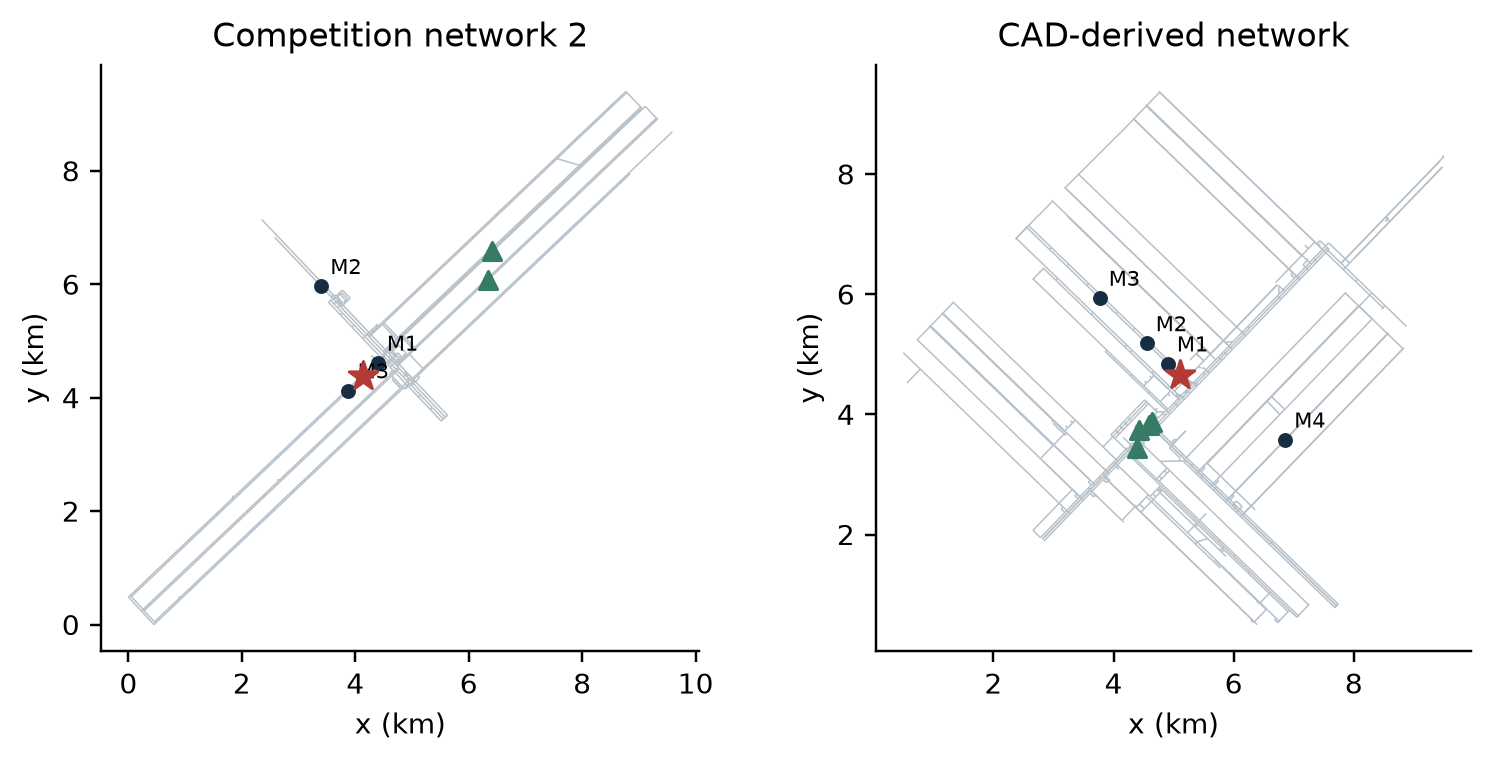
\includegraphics[width=\linewidth]{figures/networks.png}
\caption{Routing networks and base scenarios. Stars mark the inrush, triangles the designated exits, and labelled points the illustrative origins. CAD coordinates are transformed. The drawings provide geometry, not observed flood trajectories.}
\label{fig:networks}
\end{figure}

The CAD extraction joins endpoint gaps below 8 m, splits planar intersections, keeps the largest component, and adds 10--66 m shaft connectors. These rules may create or omit important connections. Roof elevations are used as a proxy for bed elevations; under the assumed constant 3 m tunnel height a uniform offset would preserve relative elevations, but actual heights are not established. The geometry has not received an independent engineering audit.

\subsection{A volume-accounting surrogate, not a hydraulic validation}
\label{sec:flood}
The routing experiments use a supplied event-driven storage-and-transfer model, described fully in Appendix~\ref{app:flood}. It assigns volume to tunnels, initially advances a shallow front, divides flow among eligible outlets, and backs water up when downstream capacity is exhausted. We use $Q=30$ m$^3$/min, height 3 m, advancing depth 0.1 m, and a mean-depth closure threshold of 0.3 m. The competition width is 4 m; the CAD width is 4.99 m. These scenario parameters do not represent measurements of an actual accident.

Unlike the original competition implementation, which simultaneously stored and retransmitted the same inflow, the surrogate accounts for stored volume and overflow. The maximum relative volume residual in the two base runs was below $3.2\times10^{-15}$. This verifies bookkeeping, not water pressure, hydraulic gradients, or local depth. In particular, equal splitting, a parent-tree transfer convention, and mean-depth closure can produce long or inaccurate hazard times.

Simultaneous events are processed in a stated lexicographic edge order. We canonicalized that order to remove dependence on workbook insertion order. Reversing the convention is a separate model sensitivity, not a different numerical tolerance. It changes some CAD closure times substantially; Section~\ref{sec:sensitivity} reports the effect.

\subsection{Origins, budgets, and withheld source locations}
In addition to the seven illustrative origins, we sample 40 non-exit vertices per network without replacement, with seed 20261025. Sampling is uniform over vertices, not tunnel length, occupancy, or worker exposure. These 80 origins are the primary denominator for aggregate single-source comparisons. All are feasible at $t_0=1$ min in the base schedules.

We evaluate nominal travel budgets $\epsilon=0,0.01,0.05,0.10$ and horizons $H=60,180$ min, as well as the unrestricted deadline. Improvements below one second are treated as numerical/non-substantive for counts; optimization itself is not rounded to seconds. The horizons are diagnostic design choices introduced to interpret the exploratory results, not operational standards or preregistered hypotheses.

For the menu experiment, each network has 16 source nodes: the base source plus 15 vertices sampled independently of outcomes using seed 20261026, excluding the base source and exits. The first eight sources are used for training and the other eight for testing. Each is paired with departure times 1, 15, 60, and 180 min. Thus every origin has 32 training and 32 test cells. Source locations are disjoint across the split. Scenario-optimal routes from test sources never enter candidate generation or menu selection.

The reported menu proportions pool test cells over the 40 sampled origins per network, conditional on an unrestricted scenario-optimal route existing. This gives 1,280 eligible cells on the competition network and 1,279 on the CAD network. Excluded infeasible cells are disclosed in the result files. Cells sharing a source are dependent, and the selected graphs are not a population sample; no binomial confidence intervals or population-level reliability claims are made.

\subsection{Verification}
The two-departure solver is compared with enumeration of all simple paths on 200 independently generated six-node directed graphs, at six delayed departures per graph. Reverse deadlines and 10\%-budget bisection brackets are checked against the same exhaustive path set. Analytic speed-switch examples, coverage examples, and ten supplied flood/routing tests are also run. All pass.

The inverse-flow scaling prediction is checked by a fresh $1.5Q$ simulation: 3,911 competition event times and 8,335 CAD event times agree with a $2/3$ scale factor to within $2.5\times10^{-15}$ in the ratios. Full paths, source identities, label counts, numerical brackets, and input hashes accompany the manuscript.

\section{Results}
\subsection{Large unrestricted gains need not buy useful time}
Table~\ref{tab:named} shows why a single headline gain is inadequate. In the competition case, the first two illustrative origins reach their maximum modelled departure deadline with at most 5\% extra nominal travel. However, the deadlines occur many days after the inrush. In the CAD case, M1 has a much shorter deadline of 4.663 min; it is already attained by the nominal route, so Corollary~\ref{cor:certificate} proves that rerouting cannot extend it in this schedule.

\begin{table}[tb]
\centering\small
\begin{tabular}{llrrrr}\toprule Network & Origin & Travel (min) & $D(P_0)$ (h) & $D_{.05}$ (h) & $D^*$ (h)\\\midrule
Competition & M1 & 11.20 & 168.75 & 254.16 & 254.16 \\
Competition & M2 & 17.13 & 206.86 & 248.53 & 248.53 \\
Competition & M3 & 18.20 & 20.27 & 20.27 & 20.27 \\
Cad & M1 & 6.39 & 0.08 & 0.08 & 0.08 \\
Cad & M2 & 8.43 & 1.97 & 1.97 & 8.18 \\
Cad & M3 & 12.96 & 1.89 & 1.89 & 47.77 \\
Cad & M4 & 14.02 & 271.16 & 271.37 & 314.95 \\
\bottomrule\end{tabular}
\caption{Illustrative origins at nominal departure 1 min. Travel is a duration; all deadlines are absolute times from inrush, in hours. $D_{.05}$ is the best deadline within a 5\% travel budget, reported at the lower bisection endpoint. Very large deadlines are features of the surrogate, not safe waiting recommendations.}
\label{tab:named}
\end{table}

For CAD M2 and M3, the maximum feasible departure is later than the deadline of the nominal route, but a 5\% travel budget does not unlock it. The extended cost curves in Figure~\ref{fig:curves} expose the distinction between an available alternative and an affordable alternative. At the extreme, the sampled curves require about 270\% extra nominal travel for M2 and 106\% for M3 near their maximum deadlines.

\begin{figure}[tb]
\centering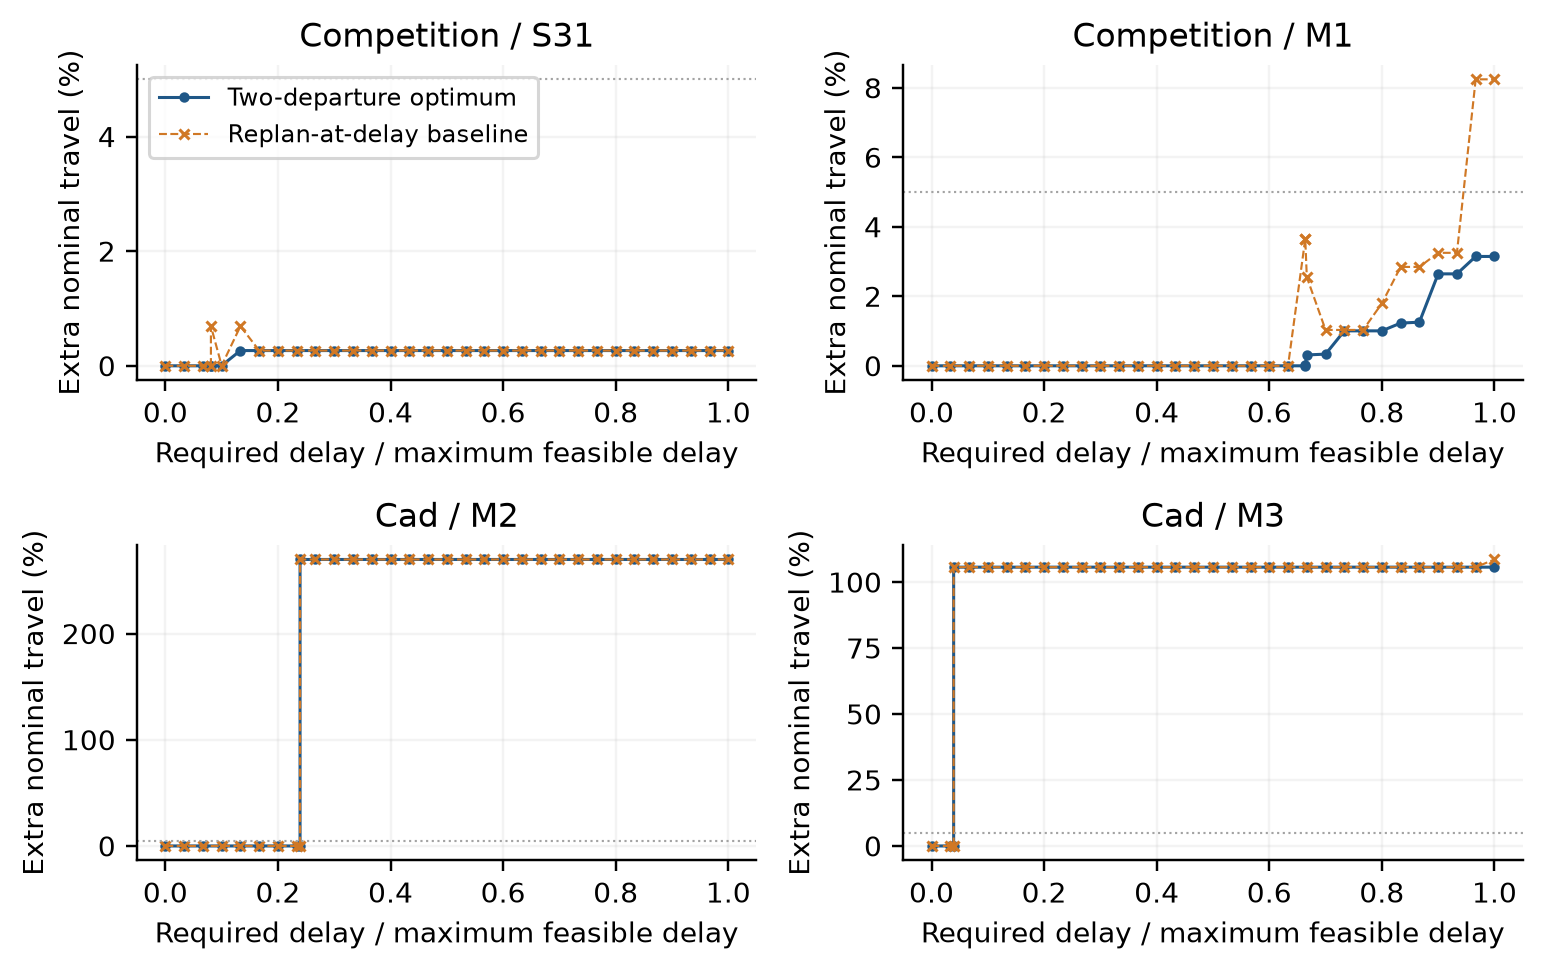
\includegraphics[width=.98\linewidth]{figures/cost_curves.png}
\caption{Cost of guaranteeing a later departure. Each point is an exact constrained query, subject to floating-point arithmetic; connecting lines guide the eye and do not claim to locate every jump. The horizontal coordinate normalizes delay by $D^*(s)-t_0$ separately for each origin. Dashed curves evaluate a route optimized at the delayed departure back at the nominal departure. The dotted horizontal line is a 5\% budget.}
\label{fig:curves}
\end{figure}

Among the 80 sampled origins, 31/40 competition origins and 32/40 CAD origins gain more than one second in unrestricted deadline under the 5\% budget. At $H=180$ min only one sampled origin benefits; at $H=60$ min none does (Figure~\ref{fig:horizons}). This is not evidence that delay tolerance is generally useless. It shows that the same output can look impressive or irrelevant depending on whether its gain occurs within the decision horizon.

The informative positive case is competition origin S31, node P0429. Its nominal travel is 26.476 min and its original route's deadline is 72.653 min. A route adding approximately 4.23 s of nominal travel extends the modelled deadline to 886.555 min. The unrestricted gain exceeds 13 hours, but the gain relevant to a 180-minute horizon is 107.347 min, and that relevant to a 60-minute horizon is zero. The large ratio should not obscure these three different quantities.

\begin{figure}[tb]
\centering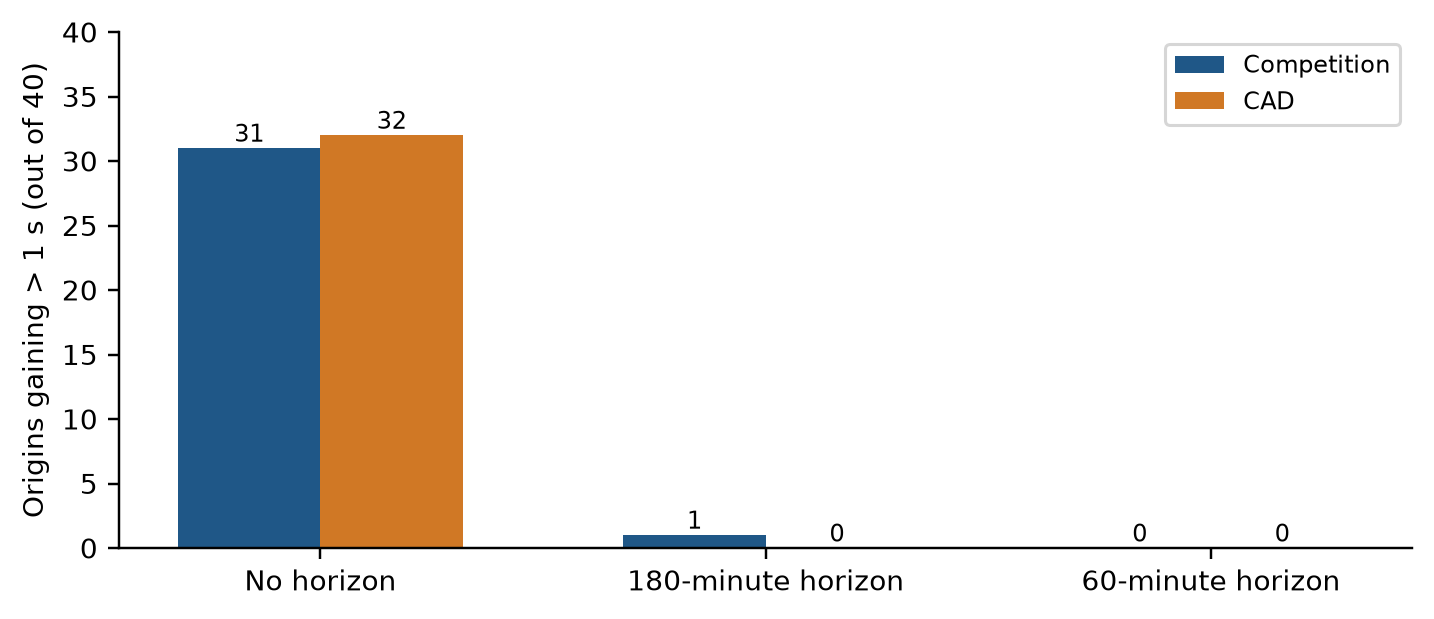
\includegraphics[width=.91\linewidth]{figures/horizons.png}
\caption{Number of sampled origins gaining more than one second under a 5\% nominal travel budget. Capping the latest useful departure time changes the interpretation of the same optimized routes.}
\label{fig:horizons}
\end{figure}

The algorithmic distinction also matters: over 260 extended-range queries, the route optimized at the delayed departure can cost up to 2.247 additional nominal minutes compared with the two-departure optimum. This is a comparison of objectives, not a claim of improved flood prediction. The largest observed number of labels retained at a node is 17; these small instances do not remove the exponential worst-case possibility.

\subsection{Small menus improve coverage modestly, and training can overfit}
Table~\ref{tab:menus} reports exact training-candidate menu selection and withheld-source evaluation. Three routes cover every training cell in which escape is possible, but do not cover every test cell. Candidate sets contain one to five routes; the median is two for the competition network and one for the CAD network.

\begin{table}[tb]
\centering\small
\begin{tabular}{lrrrrr}\toprule Network & $K$ & Train & Test & Test (\%) & Feasible (\%)\\\midrule
Competition & 1 & 1252/1279 & 1187/1280 & 92.73 & 94.84 \\
Competition & 2 & 1278/1279 & 1227/1280 & 95.86 & 97.97 \\
Competition & 3 & 1279/1279 & 1236/1280 & 96.56 & 98.59 \\
Cad & 1 & 1270/1277 & 1240/1279 & 96.95 & 98.05 \\
Cad & 2 & 1274/1277 & 1250/1279 & 97.73 & 98.83 \\
Cad & 3 & 1277/1277 & 1252/1279 & 97.89 & 98.91 \\
\bottomrule\end{tabular}
\caption{Route-menu performance on the 40 sampled origins per network. Train and Test are timely-covered/eligible cell counts. The last column counts mere feasibility, without the 10\% travel-quality restriction. $K$ is a maximum menu size; fewer routes are used when fewer candidates exist.}
\label{tab:menus}
\end{table}

Relative to the single route optimized for the base source at one minute, the three-route menu improves timely test coverage by 1.80 percentage points on the competition network (94.77\% to 96.56\%) and 0.63 points on the CAD network (97.26\% to 97.89\%). These are modest gains on ensembles with a strong baseline. The training-optimal \emph{single} route performs worse than that nominal baseline on both test sets. Optimizing one route on a small scenario collection can overfit it; preparing a menu partially offsets this fragility.

\begin{figure}[tb]
\centering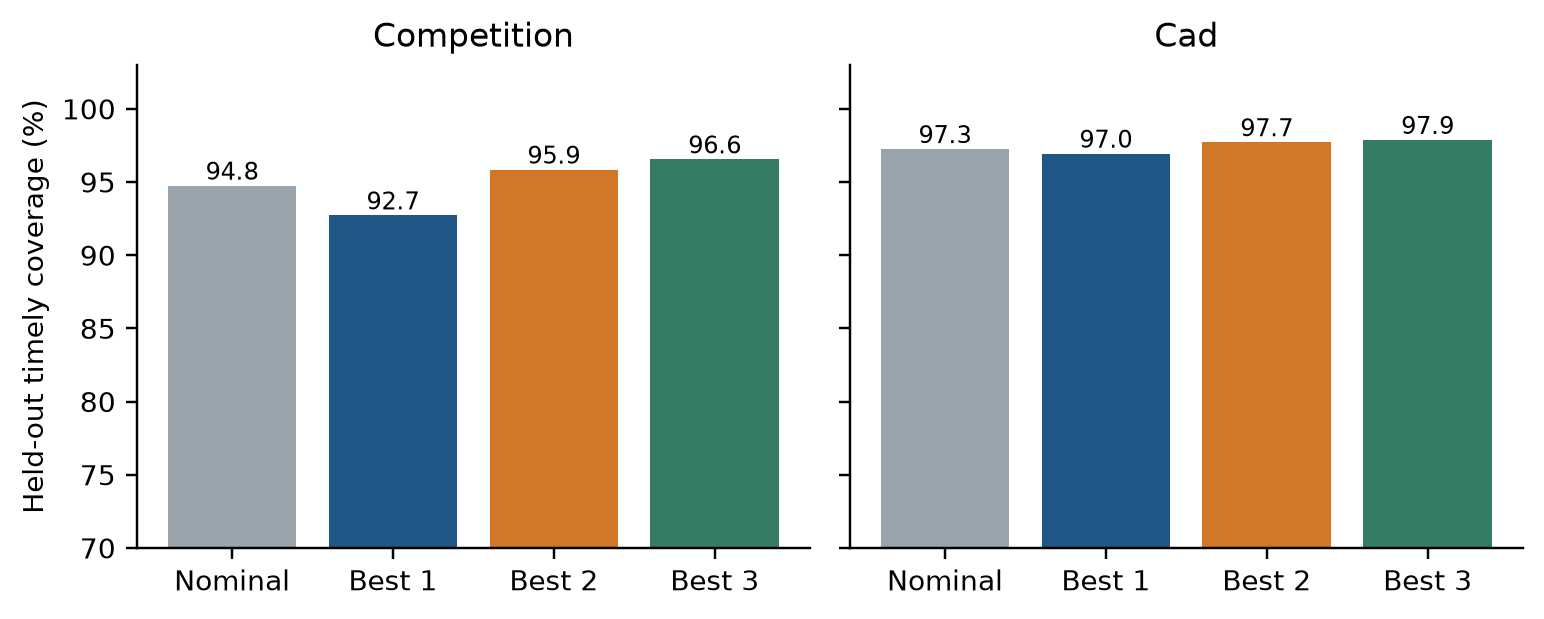
\includegraphics[width=.98\linewidth]{figures/menus.png}
\caption{Timely coverage on withheld source nodes. Nominal is the base-source fastest route at 1 min. Best $K$ is optimal on training cells within the candidate set, not on the test cells. The vertical axis starts at 70\%; exact counts are in Table~\ref{tab:menus}.}
\label{fig:menus}
\end{figure}

The menu result supports a limited interpretation: a few precomputed alternatives can improve the availability of a reasonably short route across the tested source locations. It does not establish that three routes are sufficient for all locations, nor that their correct selection is possible without information about the event. Because selection is scenario-aware in the evaluation, coverage is an upper bound on what an unspecified local decision rule would achieve.

\subsection{Sensitivity and model dependence}
\label{sec:sensitivity}
We vary inflow to 20, 45, and 60 m$^3$/min using the verified single-source scaling, hold all wet walking speeds at 1 m/s as a direction-insensitive variant, and reverse the simultaneous-event tie convention. For the 40 sampled competition origins, the unrestricted 5\%-budget improvement count remains 31; for the CAD origins it remains 32. In the competition case, increasing inflow to 45 or 60 m$^3$/min brings one improvement into the 60-minute horizon. All tested CAD variants still yield zero sampled improvements within either 60 or 180 minutes.

These aggregate counts are more stable than individual hazard times. Reversing the event convention changes some CAD closure times by as much as 38,825 s (about 10.8 h), despite volume accounting and unchanged short-horizon improvement counts. Canonical ordering makes a run reproducible; it does not resolve the physical ambiguity of simultaneous merging fronts. A calibrated hydraulic model could change the conclusions. The menu experiment uses the canonical base convention and has not been repeated over all these hydraulic variants.

\section{Discussion and limitations}
The initial question suggests a simple recommendation: accept a slightly longer route in exchange for more time to act. The results require a more selective answer. Extra nominal travel buys useful tolerance only when three conditions coincide: the baseline deadline lies within the relevant horizon, another route actually extends that deadline, and that route is affordable under the nominal travel budget. Failure of any condition makes a robustness improvement either impossible, irrelevant to the chosen horizon, or too expensive.

This interpretation also clarifies the role of precomputed routes. A menu can be useful even when a single universal route is not. But its value depends on reusable routes across scenarios and on an information mechanism for selecting among them. The experiment measures the first issue and deliberately leaves the second open. A natural next step is to define observable categories of inrush location and choose one route robust to each category, then evaluate a complete lookup or switching policy on held-out events.

Several limitations prevent safety claims. The flood surrogate is not a pressure-driven hydraulic solver; local sloping-tunnel depths, drainage, flow reversal, seals, doors, and flooding at shaft facilities are not validated. A tunnel is treated as uniformly wet once water enters it, and its closure uses average stored depth. Direction-specific wet speed is frozen to a reference direction even when later inflows merge. Canonical event priority is an explicit modelling convention. The CAD topology and interpolated roof elevations may be wrong at precisely the connections controlling a detour.

The experiments use one base inrush per network for delay optimization and only eight held-out source nodes per network for menu evaluation. Uniform vertex sampling overweights densely segmented parts of a drawing. The high nominal menu baseline indicates that many designed scenarios are not strongly discriminating. Other source distributions, heavier inflows, or different delay ranges could produce different gains. Scenario counts are not independent accident observations. The chosen 60- and 180-minute horizons illustrate interpretation, not emergency-response standards.

Finally, even the exact routing results are conditional guarantees: they concern following one route under one prescribed family of arc functions. They omit the safety of remaining at the start before departure. An availability deadline must never be interpreted as authorization to delay evacuation.

\section{Conclusion}
We formulate escape planning as a choice of how much nominal travel to exchange for a guaranteed departure interval. FIFO reduces the interval to its endpoint, but optimizing nominal arrival under that constraint generally requires two clocks. Backward deadlines provide an impossibility certificate; a constrained label search and bisection quantify the trade-off. Finite route menus extend the question to multiple flood locations without inventing accident probabilities.

The experiments show why the interpretation of robustness matters as much as its optimization. Unrestricted gains are common in these surrogate schedules, yet gains within a one-hour departure horizon are absent in the base samples. Small menus improve held-out timely coverage modestly, while a training-optimal single route can overfit. These findings support selective precomputation, explicit horizons, and honest information assumptions rather than a universal prescription to choose a slower route.

\appendix
\section{The storage-and-transfer hazard surrogate}
\label{app:flood}
This appendix specifies the simulator sufficiently to distinguish its bookkeeping from hydraulic assumptions. Each undirected tunnel has volume $V_e$, current storage rate, a reference inflow endpoint, and a mode: dry, covering, through-flow, filling, uphill ponding, full, or full conduit.

\begin{enumerate}
\item A wet node divides its incoming flow equally among nonfull outlets, excluding the tunnel currently feeding it. Level/downhill outlets are used first; uphill outlets are eligible only when there are no eligible level/downhill outlets. Elevation differences within 0.005 m count as level.
\item A dry level/downhill outlet stores flow until its volume reaches $WLh_0$. If it is fed from one endpoint and its far node is still dry, it becomes a through-flow link, wets the far node, and records a parent relation. Otherwise it continues to store water. An uphill outlet ponds until full before wetting its upper endpoint.
\item A through-flow link transfers its assigned flow without increasing its own volume. If its downstream node has no outlet, that link starts storing water instead. This separates storage from retransmission and removes the original double counting.
\item When a tunnel is full it no longer accepts storage. A source trapped behind full links is reassigned through full links to the nearest node with available storage or a backing-up parent; if none is reachable, further input is recorded as overflow. This is an algorithmic redistribution rule, not a hydraulic-head calculation.
\item Between events, storage rates are constant. The next event is the first arrival at a volume target: shallow coverage $WLh_0$, mean-depth closure $WL(0.3)$, or capacity $WLH$. Simultaneous events use the canonical edge ordering. Rates are recomputed after state changes.
\end{enumerate}

At every processed event the code checks
\[
 \frac{\left|\sum_e V_e(t)+V_{\rm overflow}(t)-\int_0^tQ(\tau)\,d\tau\right|}
 {\max\{1,\int_0^tQ(\tau)\,d\tau\}}.
\]
Closure is recorded when the mean-depth threshold is first reached. Routing begins wet-speed travel at the first entry of water, not at complete shallow coverage. This intentionally conservative spatial simplification is still not a substitute for local water depths.

For a single constant source, all rates are proportional to $Q$, while event targets are fixed volumes. With a fixed tie convention, multiplying $Q$ by $\lambda>0$ preserves the event sequence and divides all event times by $\lambda$: induct on successive target-volume events. This scale property justifies the inflow perturbations used here. It does not extend unchanged to multiple sources with unscaled activation delays or time-dependent drainage.

Flooding is run on the graph split only at the inrush. Origins inserted afterward inherit the original directed arc schedule on each subarc. This preserves exact traversal through those observation splits and avoids changing storage dynamics merely by adding a miner's location. It does not establish invariance of the flood surrogate to arbitrary remeshing of the underlying CAD network.

\section{Verification, numerical conventions, and reproducibility}
The accompanying directory contains \texttt{code/}, \texttt{data/}, \texttt{results/}, and \texttt{figures/}. The two-departure method is in \texttt{robust.py}; \texttt{run.py} produces budget results; \texttt{diagnostics.py} checks scaling and model variants; \texttt{menus.py} generates the source-split menu experiment. The manuscript tables and figures are generated from those outputs, rather than transcribed from a prior draft.

Five new tests include exhaustive comparison of 1,200 constrained queries on 200 random directed graphs, comparison of reverse and budget deadlines with all simple paths, and exact small-menu examples. Ten inherited tests cover single tunnels, series, forks, loops, elevation rules, multiple sources, volume accounting, FIFO, inverse arrival maps, and shortest paths versus enumeration. This is algorithm verification, not validation against observed flooding.

Closure comparisons use a $10^{-9}$ s numerical allowance inherited from the routing model; reverse-bound pruning uses $10^{-8}$ s. Label dominance uses direct componentwise comparisons without heuristic tolerances. Budget bisection uses a 0.01 s final bracket and a $10^{-8}$ s objective allowance. Gains counted in tables exceed one second, far above these allowances. Raw paths and lower/upper deadline brackets are retained.

The additional 40 origins in each network are stored explicitly, as are all menu source nodes and train/test assignments. Input and source-code SHA-256 hashes identify the computation. Portable JSON routing schedules permit routing results to be inspected independently of the flood implementation. Pickle caches are local acceleration files and are not required for a fresh run.

The competition workbook and CAD-derived network accompany this local research package. The original CAD drawing and coordinate-transform key do not. No public repository, release permission, or independently verified mine provenance is asserted. The source geometry is an anonymized derivative supplied for this study. The manuscript is a working research draft; the code, mathematical development, and exposition were prepared with AI assistance and require author review before external circulation.

\begin{thebibliography}{9}
\small
\setlength{\itemsep}{3pt}
\setlength{\parskip}{0pt}
\bibitem{cumcm}
China Society for Industrial and Applied Mathematics.
\emph{CUMCM 2025, Problem D: Mine Water-Inrush Propagation and Escape Planning}.
Problem statement and Attachment 2, 2025. Supplied competition materials;
\url{https://en.mcm.edu.cn/}.

\bibitem{dean}
B. C. Dean.
\emph{Shortest Paths in FIFO Time-Dependent Networks: Theory and Algorithms}.
Technical report, Massachusetts Institute of Technology.
\url{https://people.csail.mit.edu/bdean/tdsp.pdf}.

\bibitem{orda}
A. Orda and R. Rom.
Shortest-path and minimum-delay algorithms in networks with time-dependent edge-length.
\emph{Journal of the ACM}, 37(3):607--625, 1990.
\url{https://doi.org/10.1145/79147.214078}.

\bibitem{ichoua}
S. Ichoua, M. Gendreau, and J.-Y. Potvin.
Vehicle dispatching with time-dependent travel times.
\emph{European Journal of Operational Research}, 144(2):379--396, 2003.
\url{https://doi.org/10.1016/S0377-2217(02)00147-9}.

\bibitem{martins}
E. Q. V. Martins.
On a multicriteria shortest path problem.
\emph{European Journal of Operational Research}, 16(2):236--245, 1984.
\url{https://doi.org/10.1016/0377-2217(84)90077-8}.

\bibitem{fischetti}
M. Fischetti and M. Monaci.
Light robustness.
In \emph{Robust and Online Large-Scale Optimization}, LNCS 5868, pp. 61--84, 2009.
\url{https://doi.org/10.1007/978-3-642-05465-5_3}.

\bibitem{goerigk}
M. Goerigk, S. He{\ss}e, M. M{\"u}ller-Hannemann, M. Schmidt, and A. Sch{\"o}bel.
Recoverable robust timetable information.
In \emph{ATMOS 2013}, OASIcs 33, pp. 1--14, 2013.
\url{https://doi.org/10.4230/OASIcs.ATMOS.2013.1}.

\bibitem{nemhauser}
G. L. Nemhauser, L. A. Wolsey, and M. L. Fisher.
An analysis of approximations for maximizing submodular set functions---I.
\emph{Mathematical Programming}, 14:265--294, 1978.
\url{https://doi.org/10.1007/BF01588971}.
\end{thebibliography}
\end{document}
